\documentclass{article}
\usepackage[utf8]{inputenc}
\usepackage{graphicx}
\usepackage{float}
\usepackage[numbers]{natbib}
\usepackage{amsmath}
\title{Projeto de Doutorado}
\author{Carlos Miguel Moreira Gonçalves}

\begin{document}

\maketitle

\section{Resumo}

O rápido crescimento da área urbana sem o devido cuidado pode gerar diversos problemas economicos, sociais, ambientais e pode comprometer a estrutura a malha urbana. A previsão de quão vantajoso é uma mudança no conjunto de vias seja com reformas ou adicionadas pode otimizar o gasto em trânsito, que pode ser realocado em outras áreas essenciais, diminuição na poluição ou redução de congestionamentos. Através de modelagem computacional, esse projeto propõe simulações para entender como congestionamentos se propagam em diferentes cidades e quais são as vias que mais podem ser mais frágeis a engarrafamentos. Além disso, em geral para esse estudo é necessário o conhecimento de uma matriz Origem-Destino (OD) que é muito difícil de ser coletada devido à um grandes esforço na sua coleta e nos problemas éticos que isso pode causar. Para evitar isso será avaliado algoritmos que a aprtir de fluxos coletados da API do \textit{Google Maps} seja possível conseguir a matriz OD. Portanto, esse trabalho visa contribuir para uma melhor entendimento do fenômeno de congestionamento e como é sua propagação dentro da cidade o que pode acarretar em um novo conhecimento sobre a física de percolação nesse contexto.

\newpage

\section{Introdução}

%//! Introdução ao tema!


A escalada da urbanização \cite{urbanization} em tempos recentes desencadeou uma série de investimentos significativos na expansão e melhoria das ruas e avenidas, visando facilitar a locomoção nas cidades. Tais investimentos, caracterizados por aportes financeiros substanciais e extensos períodos dedicados à infraestrutura e finalização das obras, refletem o esforço para acompanhar as demandas de uma população em crescimento, como ilustrado na evolução da urbanização em Fortaleza na Figura \ref{fig:urbanizacao}. No entanto, a ausência de uma análise meticulosa da infraestrutura viária pode acarretar uma série de consequências adversas, incluindo a proliferação de congestionamentos, o aumento do nível de estresse entre motoristas e passageiros \cite{Hegewald2020,Adli2017}, a elevação do risco de acidentes e, consequentemente, um incremento nas emissões de gases nocivos ao meio ambiente \citep{Wang2018}. Esses efeitos colaterais não apenas comprometem a eficácia dos investimentos em mobilidade urbana, mas também impactam negativamente a qualidade de vida nas cidades.

\begin{figure}[H]
    \centering
    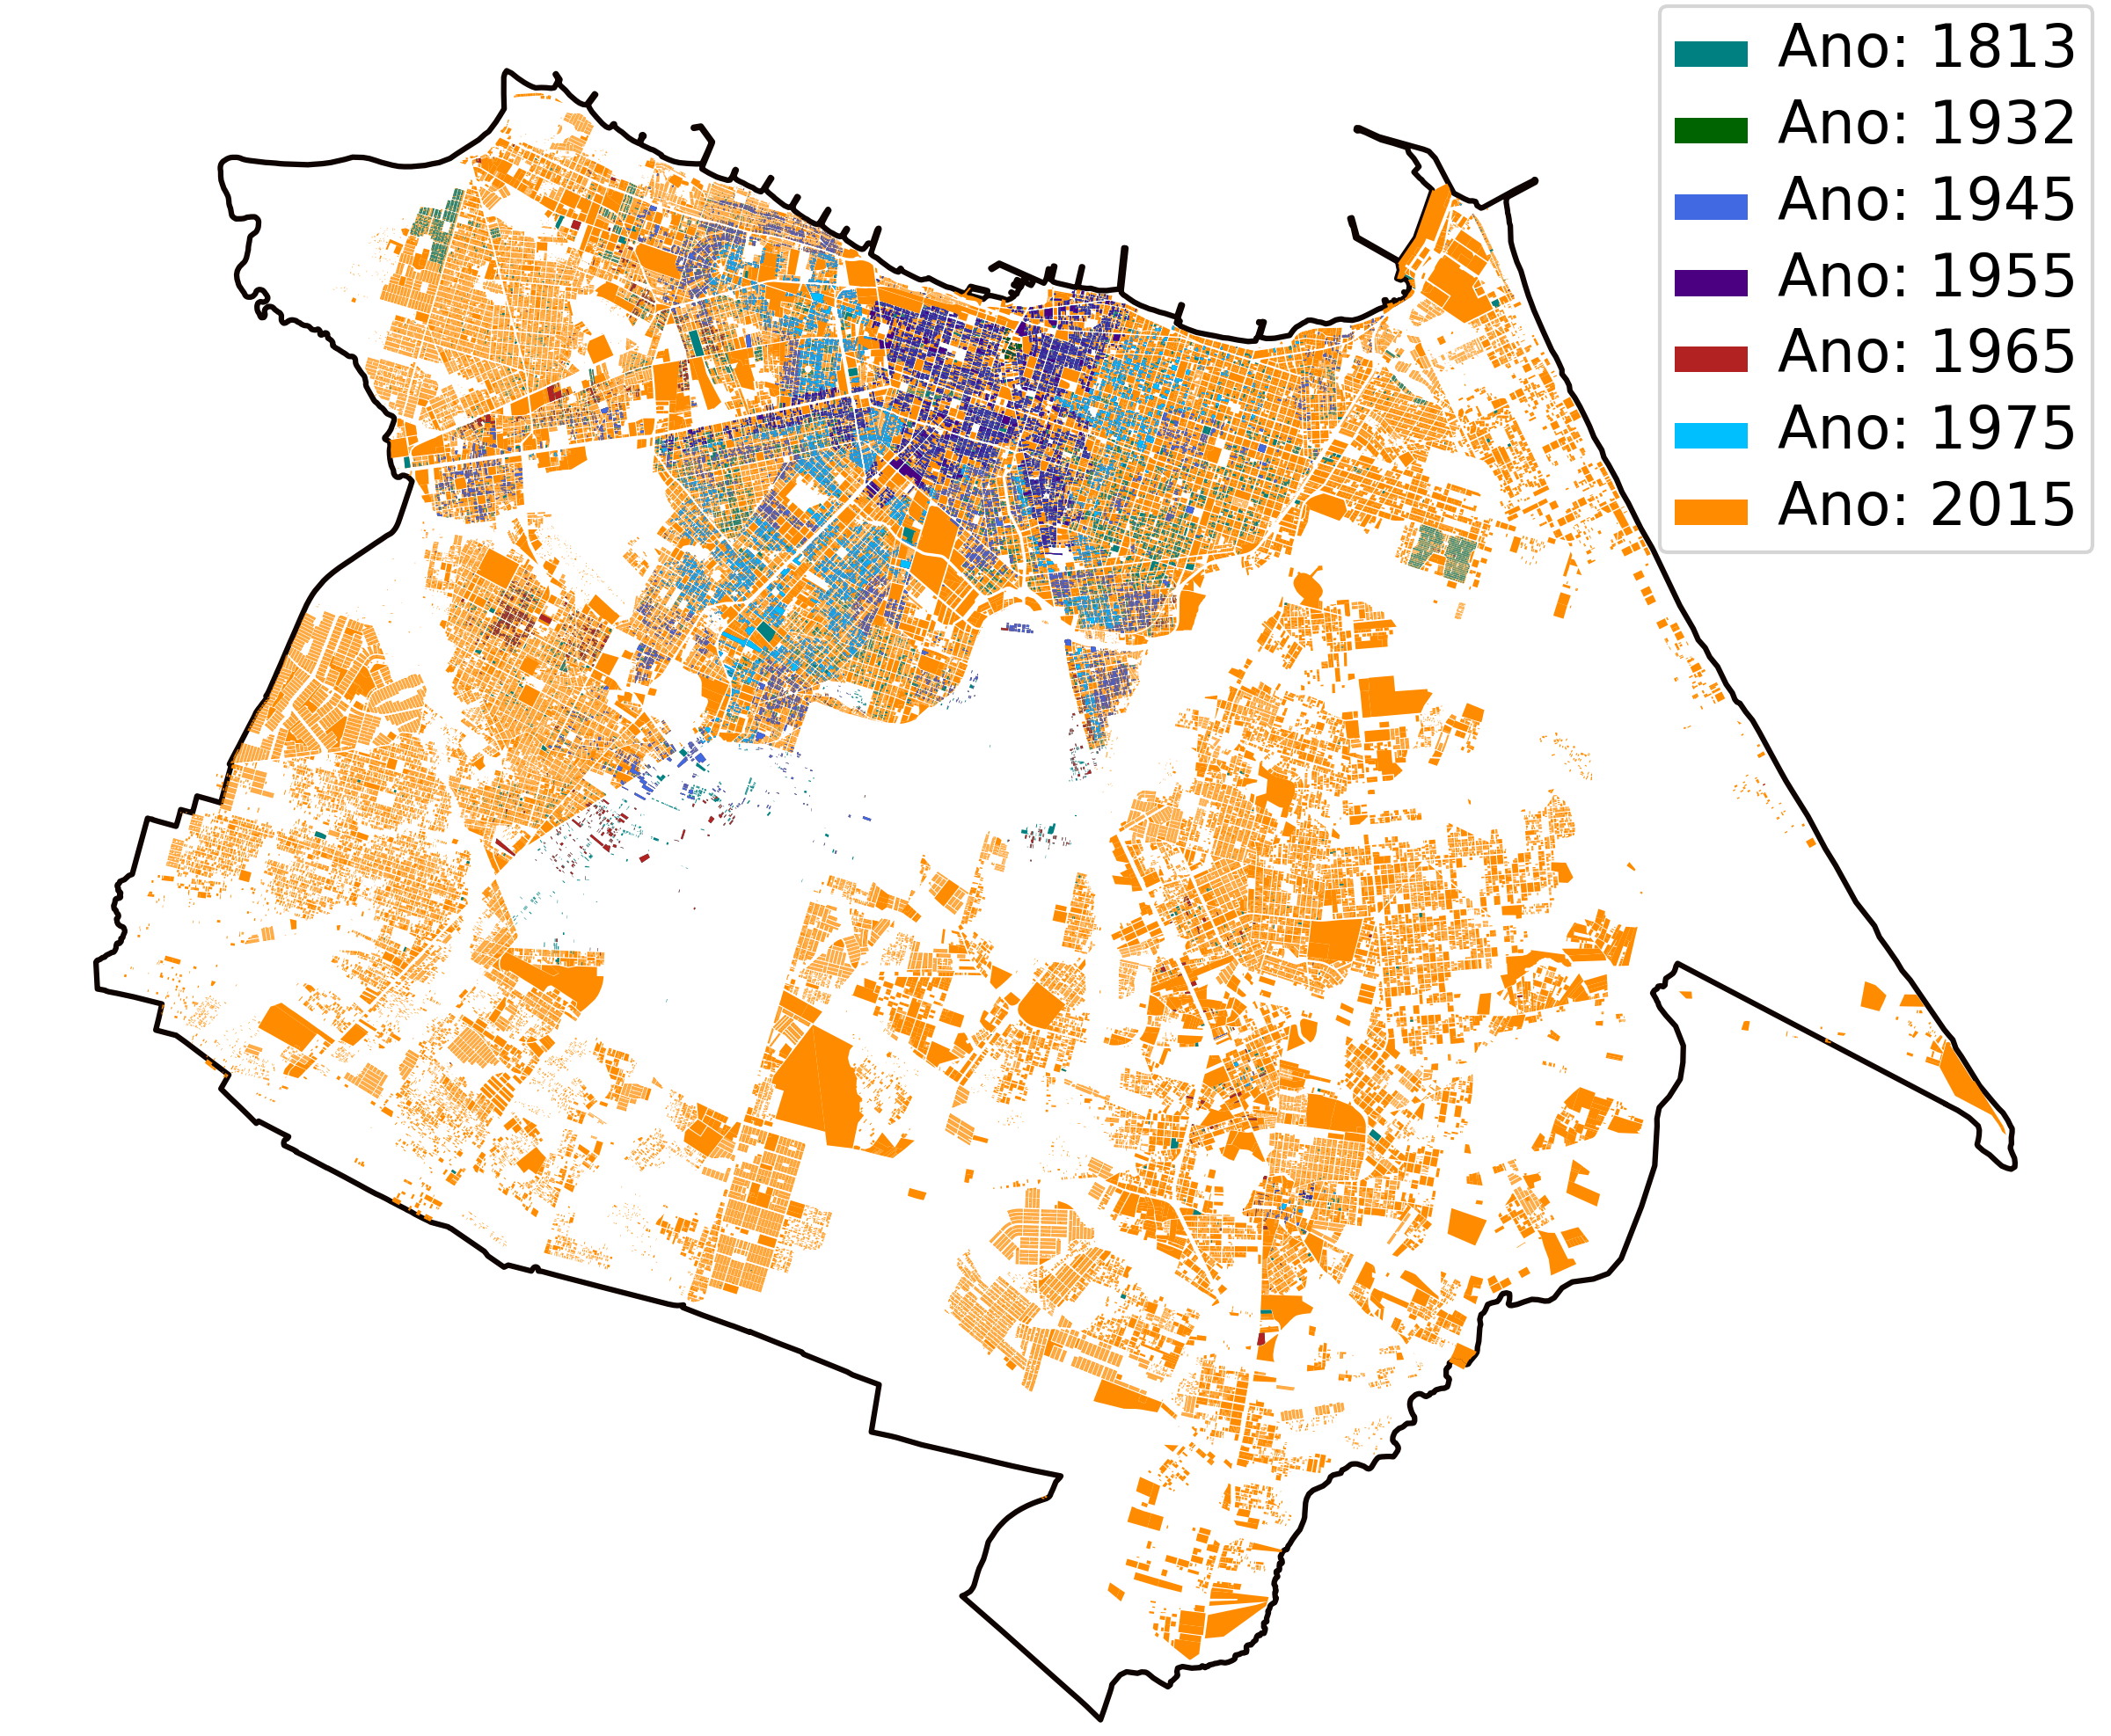
\includegraphics[width=0.7\textwidth]{img/urbanizacao.png}
    \caption{Evolução temporal da urbanização na cidade de Fortaleza.}
    \label{fig:urbanizacao}
\end{figure}

%//! Explicação da abordagem computacional!

Neste contexto, a modelagem computacional é uma ferramenta viável para abordar esses desafios urbanos complexos. Através de simulações precisas, é possível antecipar os impactos decorrentes de intervenções na infraestrutura viária, como a construção de novas vias, melhorias em rotas existentes, ou as consequências de obstruções temporárias provocadas por eventos climáticos adversos ou acidentes. O interesse por esta questão também se origina na presença de fundamentos físicos intrínsecos, tais como a lei da conservação do fluxo e o princípio de minimização de uma função de custo associada, além da manifestação de fenômenos críticos caracterizados por transições de fase entre estados de fluxo livre e congestionamento. 

%//! Explicação da transição de fase

Transições de fase representam transformações fundamentais que ocorrem em vários contextos, desde fenômenos físicos, como a mudança de estados da matéria, até aplicações em processos biológicos e a dinâmica de atribuição de tráfego, onde sistemas experimentam mudanças abruptas de estado. Essas mudanças abruptas são quantificáveis através de expoentes críticos, os quais não dependem da dimensionalidade do sistema. Essa independência dimensional sugere que problemas distintos, quando compartilham expoentes críticos similares, podem ser agrupados em uma categoria comum denominada classe de universalidade. 
\citet{Li2014,Zeng2018} exploraram a dinâmica do tráfego na rede viária de Pequim, revelando uma transição de fase. Eles criaram um parâmetro que determina a capacidade de uma via para acomodar o fluxo de veículos. Descobriram que há um valor crítico, que varia com o tempo, no qual emerge o fenômeno da percolação. \citet{Ambhl2023} aprofundaram a análise ao investigar as redes viárias de cinco grandes metrópoles, focando na evolução do maior conglomerado urbano e encontraram uma forte correlação entre a percolação do congestionamento e o fluxo médio da rede.

No entanto, a aplicação desta metodologia enfrenta obstáculos intrínsecos. Em primeiro lugar, a determinação das variáveis que um indivíduo considera ao escolher um percurso dentro do tecido urbano permanece incerta; não está claro se, ou como, as pessoas buscam otimizar seus trajetos em termos de tempo, custo ou conforto. Em segundo lugar, a velocidade de fluxo nas vias urbanas é diretamente influenciada pela densidade de tráfego, tornando a previsão do tempo de percurso uma questão dinâmica, sujeita a flutuações constantes em função do volume de veículos e por último a quantidade de dados disponíveis.

%//! Explicação da otimização do motorista

Assim como a corrente elétrica naturalmente encontra o caminho de menor resistência numa rede de resistores, e o fluido se desloca através do caminho de menor impedância em um meio poroso, seguindo a Lei de Darcy \citep{darcy}, os motoristas em uma rede urbana também buscam otimizar seus percursos. No entanto, ao contrário dos sistemas físicos regidos por leis bem definidas, o processo de decisão dos motoristas incorpora uma complexidade substancialmente maior. Esta complexidade deriva da diversidade de fatores que podem influenciar a escolha de uma rota, que vão além do mero cálculo de eficiência temporal ou de deslocamento. A seleção de um caminho pode ser afetada por aspectos como congestionamento, conhecimento da área, preferências pessoais, e até condições momentâneas, como o estado do tempo ou o humor do motorista resultando em trajetórias significativamente distintas daquelas focadas no benefício individual, ou uma abordagem altruísta, voltada para o bem-estar coletivo da sociedade. 

\citet{Anarchy} estudaram a razão do tempo considerando a otimização egoísta pelo tempo otimizando a sociedade e como esse valor se comporta em diferentes cidades e em modelos tradicionais de redes. 

%//! Fluxo em vias

Outro impasse nessa modelagem é a influência direta da densidade de tráfego sobre a velocidade de fluxo nas vias urbanas, à medida que a concentração de veículos aumenta em uma via, a mobilidade tende a ser comprometida, levando a uma redução na velocidade média e, eventualmente, a situações de congestionamento. Nesse contexto, para modelagem é utilizado, tradicionalmente, a função de Bureau of Public Roads (BPR) \citep{Dial2006,Anarchy,Ambhl2023}. A função BPR (Equação \ref{eq:BPR}) determina o tempo $l_{i,j}$ entre dois pontos $i$ e $j$ que depende da velocidade limite da rua $v_{i,j}$ do fluxo $f_{i,j}$, da distância $d_{i,j}$ entre $i$ e $j$ e da capacidade $p_{i,j}$ com dois parâmetros $\alpha = 0.2$ e $\beta = 10 $\citep{Anarchy}. Essa função é aproximadamente constante para valores de $f_{i,j} < p_{i,j}$ porém é altamente não linear quando $f_{i,j} \geq p_{i,j}$ e rapidamente tende a infinito.

\begin{equation}
    l_{i,j} = \frac{d_{i,j}}{v_{i,j}}\left(1 + \alpha\left(\frac{f_{i,j}}{p_{i,j}}\right)^{\beta} \right)
    \label{eq:BPR}
\end{equation}

\begin{figure}[H]
    \centering
    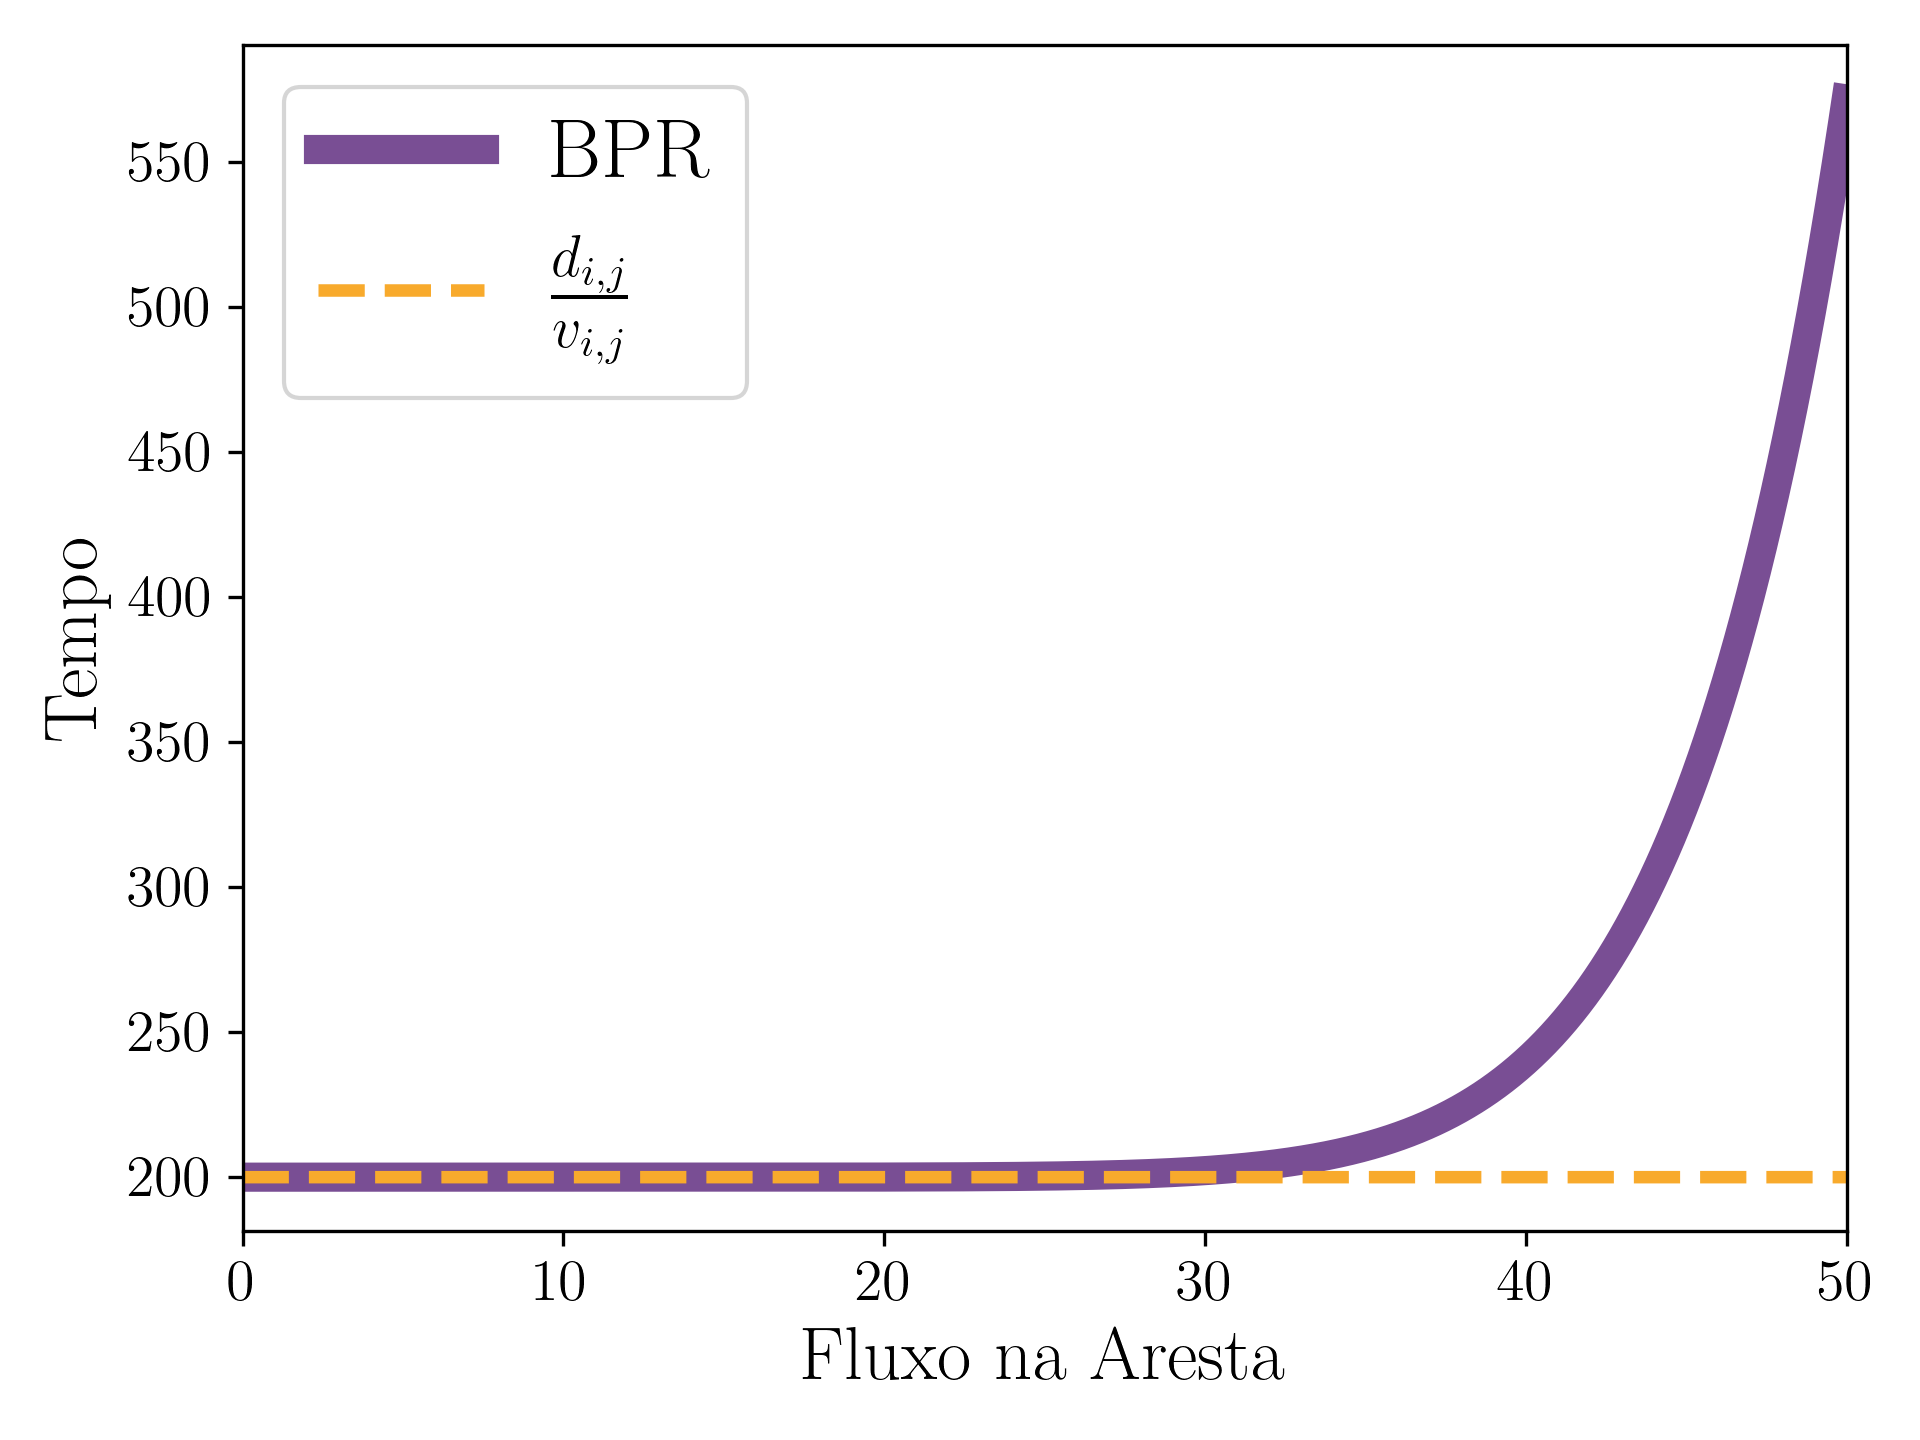
\includegraphics[width=0.7\textwidth]{img/BPR.png}
    \caption{Comportamento da Função BPR com o incremento de fluxo.}
    \label{fig:BPR}
\end{figure}

%//! Coleta de dados

Por fim, a obtenção dos dados, apresenta desafios significativos em termos de sensibilidade temporal, uma vez que as condições de tráfego são altamente dinâmicas e sujeitas a variações diárias, sazonais e devido a eventos não regulares. Além disso, há questões morais intrínsecas à coleta e ao uso desses dados, particularmente no que se refere à privacidade dos indivíduos. As informações de localização e padrões de movimento, por exemplo, podem revelar detalhes sobre a vida das pessoas, levantando preocupações éticas sobre como esses dados são coletados, armazenados e utilizados. \citet{Simini2012} utilizaram um modelo para tentar estimar, dado uma conexão entre cidades dos Estados Unidos, o número de pessoas que trafegam entre as duas cidades.

Os principais trabalhos que estudam tráfego precisam, majoritariamente, de uma matriz chamada de Origem-Destino (OD) que cada elemento representa quantas pessoas saem de uma região para outra. Utilizando essa matriz, grafo da região em estudo e algoritmos de programação não linear \cite{LeBlanc1975} conseguem obter o fluxo de cada aresta do grafo. Uma das mais estudadas formulações desse problema é assumindo que os indivíduos otimizam o seu próprio tempo, sem se preocupar se isso será pior para rede como um todo e devemos assumir a conservação de fluxo de veículos. Seja $G$ um grafo composto por um conjunto $N$ de nós e um conjunto $A$ de arestas, o problema que deve ser resolvido é:
\   
\begin{align}
    \min_{x} \sum_{(i,j) \in A} l_{i,j}\left(\sum_{s = 1}^{p}f^p_{i,j}\right),\\
    \text{sujeito a:} OD(j,s) = \sum_{(j,k) \in A}f^s_{j,k} - \sum_{(i,j) \in A}f^s_{i,j},\\
    f_{i,j} = \sum_{p}f^p_{i,j} \forall (i,j) \in A ,\\
    f^s_{i,j} \geq 0 \forall s\\
\end{align}

na qual $OD(j,s)$ é a quantidade de indivíduos que desejam sair do nó $j$ e irem para o nó $s$, $f^s_{i,j}$ representa o fluxo que passa entre a aresta $(i,j)$ e que tem o intuito de chegar em $s$. A equação (3) representa que ao passar por um nó, se existe saldo significa que existem pessoas querendo ir de $j$ para $s$.

Entretanto, como explicado anteriormente a matriz OD e até os valores $f^p_{i,j}$ são difíceis de serem coletados e são confidenciais. Contudo com o auxílio do \textit{Google Maps} é possível ter acesso ao fluxo em determinada rua por meio da sua API e assim pode-se tentar encontrar a matriz OD utilizando outras técnicas de otimização \cite{spiess1990gradient,turnquist1979estimation,spiess1987maximum}.

Portanto, neste projeto, é proposto um estudo sobre o comportamento de congestionamento em cidades, a partir de dados de Matrizes Origem-Destino, e como ele se propaga dentro da malha viária. Em paralelo a isso também será analisado a viabilidade de algoritmos para obtenção dessas matrizes em outras cidades a partir do fluxo de APIs do \textit{Google Maps}, pois isso expandiria o trabalho para mais cidades e para um estudo ao longo do tempo.

%//! Proposta do trabalho 

\newpage
\section{Objetivos}

Este projeto propõe uma investigação dos modelos de distribuição de tráfego em redes viárias, com o intuito de compreender as dinâmicas que governam o movimento e a alocação de indivíduos em diferentes vias. Essa investigação será conduzida através da aplicação de diversas métricas e técnicas de otimização, visando não apenas desvendar a distribuição baseadas em matrizes Origem-Destino, mas também explorar a possibilidade de reconstruir essas matrizes a partir dos fluxos observados na rede. Outrossim, o estudo pretende examinar os efeitos dos congestionamentos no comportamento geral do fluxo, proporcionando uma compreensão mais refinada de como as interrupções e as variações de capacidade impactam a distribuição de tráfego. A seguir, os objetivos específicos são detalhados:

\begin{enumerate}
    \item Investigar e analisar modelos matemáticos e computacionais que descrevem a distribuição de indivíduos em redes de transporte. Este objetivo inclui a aplicação e o desenvolvimento de métricas para avaliar a eficiência, a equidade e a sustentabilidade dos padrões de tráfego resultantes.
    \item Explorar a viabilidade de inferir matrizes Origem-Destino a partir de dados de fluxo observados, utilizando técnicas inversas e métodos de otimização. Este aspecto é crucial para melhorar as estratégias de planejamento e gestão de tráfego, especialmente em contextos onde os dados de origem-destino não estão diretamente disponíveis.
    \item Avaliar como os congestionamentos alteram os padrões de fluxo dentro da rede, utilizando modelagem dinâmica e simulações para compreender as mudanças no comportamento dos usuários e na eficiência geral da rede sob condições variáveis de tráfego.
\end{enumerate}

\newpage

\section{Métodos}

\begin{itemize}
    \item \textbf{Coleta de Dados:} a partir de dados de cidades obtidos através da API do Google Maps, ou recorrendo a conjuntos de dados publicados em artigos acadêmicos, que podem ser representados sob a forma de matrizes Origem-Destino ou como fluxos de tráfego específicos de uma área urbana em determinados períodos, daremos início às nossas análises. Além disso o site OpenStreetMap disponibiliza a partir da sua biblioteca do Python o shapefile de qualquer cidade.
    \item \textbf{Análise dos Dados:} A exploração desses conjuntos de dados pode ser realizada sob múltiplas perspectivas. Para os dados organizados em matrizes Origem-Destino, é factível derivar os correspondentes fluxos de tráfego mediante a aplicação de modelos consolidados na literatura científica, os quais podem ser adaptados e otimizados levando em consideração as singularidades de cada indivíduo na rede. Quanto aos dados relativos a fluxos específicos, abre-se a possibilidade de tentar reconstruir as matrizes OD, pois a construção dessas matrizes é muito custosa.
    \item \textbf{Estudo de Engarrafamentos:}  Analisando a malha viária urbana e a distribuição de fluxos em cada via, é possível investigar a extensão do impacto que diversas interrupções — como obras de infraestrutura, congestionamentos ou inundações — exercem sobre as rotas adjacentes. Essa análise permitirá identificar não apenas as cidades mais vulneráveis a essas perturbações, mas também aquelas vias específicas que, quando obstruídas, têm maior potencial de desencadear efeitos em cascata, levando a engarrafamentos generalizados. 
    \item \textbf{Impactos de Falhas Semafóricas:} durante períodos chuvosos, é frequente a ocorrência de falhas em semáforos, provocando uma dinâmica em que pedestres e motoristas, enfrentando cruzamentos com sinais inoperantes, hesitam em ceder passagem, gerando congestionamento na rua perpendicular. Essa situação pode ser meticulosamente modelada para compreender as interações e o comportamento dos usuários da via, permitindo identificar quais semáforos demandam atenção prioritária em termos de manutenção preventiva. Além disso, diante da iminência de falhas, a implementação de uma estratégia proativa, que inclua a designação de pessoal para gestão do trânsito, pode mitigar o impacto negativo desses eventos no fluxo veicular e na segurança dos usuários da via.
\end{itemize}

\newpage

\section{Resultados Esperados e Cronograma}

Espera-se desenvolver uma análise sobre o comportamento de congestionamentos dentro de cidades e sua evolução, como se comporta os fluxos com esse congestionamento e quando existem falhas nos semáforos e o estudo de modelos para encontrar as matrizes OD pelos fluxos dentro da rede.

\begin{itemize}
    \item \textbf{Primeiro Ano}:
    \begin{itemize}
        \item Concluir as cadeiras obrigatórias;
        \item Analisar os métodos de otimização para dado uma matriz OD encontrar os fluxos na rede;
        \item Analisar os métodos de otimização para dado fluxos em redes encontrar a respectiva matriz OD;
    \end{itemize}
    \item \textbf{Segundo Ano}:
    \begin{itemize}
        \item Concluir as cadeiras optativas e estágio a docência;
        \item Entender o funcionamento da API do Google Maps e obter as matrizes OD em diferentes cidades;
        \item A partir das matrizes OD fazer os primeiros estudos sobre congestionamento;
    \end{itemize}
    \item \textbf{Terceiro Ano}:
    \begin{itemize}
        \item Escrita da qualificação do doutorado;
        \item Investigar a falha em semáforos dentro da rede viária, como os fluxos são alterados e quais os semáforos que podem gerar mais defeitos utilziando-se métricas em redes;
        
    \end{itemize}
    \item \textbf{Terceiro Ano}:
    \begin{itemize}
        \item Fazer as últimas análises dos resultados;
        \item Defender a tese;
    \end{itemize}
\end{itemize}


\newpage

\bibliographystyle{unsrtnat} % Use o estilo unsrtnat
\bibliography{reference.bib}
\end{document}
